\chapter{Komponenten}
\section{Webcrawler}
\subsection{Beschreibung der Technologie}
\subsubsection{Apache Storm}
StormCrawler basiert auf Apache Storm, einem Opensource Framework zur verteilten Stream-Verarbeitung.
Die Architektur von Apache Storm basiert auf den folgenden Komponenten:
\begin{itemize}
	\item Spout - Komponente zum Einlesen von Daten-Streams
	\item Bolt - Komponente zum Verarbeiten von Daten-Streams
	\item Tupel - Datensatz, welcher zwischen den Komponenten weitergegeben wird
	\item Topologie - Ein Netz bestehend aus Spouts und Bolts
\end{itemize}
Jede Komponente ist als eigene Java-Klasse definiert und beinhaltet zwingend die folgenden Methoden:
\begin{itemize}
	\item execute() - Ausführen des Tasks der Komponente
	\item declareOutputFields() - Definition des Ausgabeschemas des Tupels
\end{itemize}
In einer Topologie werden verschiedene Spouts und Bolts miteinander verknüpft, um einen Prozess durchzuführen, wie in \cref{fig:topology} gezeigt wird.
\begin{figure}[H]	
	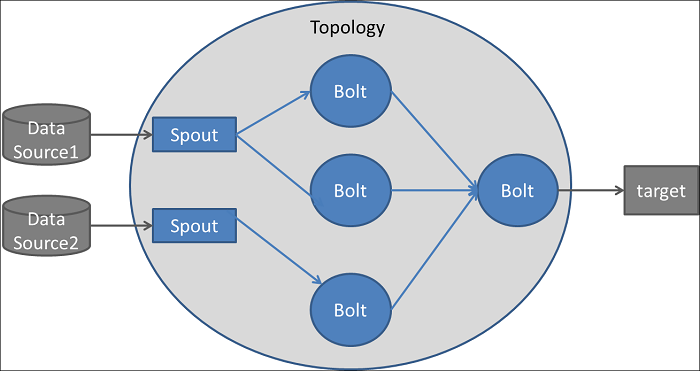
\includegraphics[width=0.8\columnwidth,keepaspectratio]{img/storm-topology.png}
	\caption{Beispieltopologie\\ Quelle: https://dzone.com/articles/apache-storm-architecture}
	\label{fig:topology}
\end{figure}
Dabei hat der Spout die Aufgabe, Daten aus einer Quelle (z.B. Datei, Datenbank, Array) einzulesen und daraus ein Tupel zu bilden.
Dieses Tupel wird an die weiteren Bolts der Topologie weitergegeben und von diesen verarbeitet.
Diese Verarbeitung muss nicht seriell stattfinden, die Topologie kann auch Gabelungen beinhalten, die dementsprechend Bolts benötigen, welche entscheiden, an welchen Folge-Bolt das Tupel weitergegeben werden soll.
Zudem ist eine Webapplikation verfügbar, die eine Übersicht über die Informationen wie eine Topologieübersicht, der Status der jeweiligen Komponenten sowie Fehlermeldungen anzeigt.
\subsubsection{StormCrawler SDK}
StormCrawler ist ein Opensource Software Development Kit, welches auf Apache Storm aufbaut und in Java entwickelt wurde.
Er dient als Baukasten, um einen Webcrawler aufzubauen, der skalierbar, stabil und sehr effizient ist.
Er beinhaltet verschiedene Spouts und Bolts, die explizit zum Crawlen von Websites vorgefertigt wurden.
Zudem berücksichtigt er die Regeln des Webcrawling, also Meta-Tags oder Robot.txt Dateien, welche deklarieren, ob eine Website gecrawlt werden darf.
Weiter ist er so eingerichtet, dass Webpages derselben Website mit einer Zeitverzögerung abfragt, damit diese nicht überlastet werden.
StromCrawler ist standardmässig so eingerichtet, dass nur Webpages desselben Hosts gecrawlt werden.
\subsubsection{Docker}
\paragraph{Docker Einführung}
Docker besitzt verschiedene Bedeutungen. Docker kann sich auf den Namen der Firma Docker Inc."fussnote" beziehen oder auf die eigentliche Software.
In diesem Kontext wird Docker als die Software zum Erstellen von Linux-Containern verwendet.
Mithilfe von Docker können ressourcenarme, modulare virtuelle Maschinen erstellt werden, welche auch Container genannt werden.
Diese Container können dann einfach kopiert, ersetzt oder auf einem anderen System verwendet werden.
\footnote{\url{https://www.redhat.com/de/topics/containers/what-is-docker}}

\paragraph{Unterschiede zu Virtual Machines}
Im Gegensatz zu kompletten Virtual Machines (VM) besitzen Container einen deutlich kleineren Speicherfootprint.
VMs abstrahieren physische Hardware zu virtuellen Hardwarekomponenten. Auf diesen virtuellen Hardwarekomponenten können dann Betriebssysteme
und Software betrieben werden ähnlich wie auf der physischen Hardware.
Container abstrahieren jedoch auf Betriebssystemebene.
Dadurch bekommt man eine virtuelle Variante des physischen Host-Systems, auf dem man anschliessend Software und Abhängigkeiten betreiben kann.
Für die Containerisierung ist es notwendig, dass das Host-System eine Linux-Distribution ist.
\footnote{\url{https://wirtschaftslexikon.gabler.de/definition/hardware-virtualisierung-53364}}

\paragraph{Linux-Container}
Linux-Container verwenden den Linux-Kernel und seine Funktionen um Isolation der einzelnen Prozesse zu realisieren.
Durch die Isolation der Prozesse können diese unabhängig voneinander ausgeführt werden,
was die Auslastung des Host-Systems verbessert und ebenfalls die Sicherheit des Gesamtsystems erhöht.
Der Vorteil von Containern ist, dass alle Abhängigkeiten mit der ausführbaren Software in den Container gepackt werden können und somit jede
Umgebung, die den gleichen Container verwendet, auch den gleichen Softwarestand besitzt.
Dadurch wird die Software auf jeder Umgebung identisch ausgeführt.
Docker selbst baut auf der LXC-Technologie, eine Technologie zur Virtualisierung von Linux-Container auf Betriebssystemebene, auf,
erweiterte diese Technologie jedoch für das einfachere Erstellen, Warten und Versionieren von den erstellten Docker Containern.
\footnote{\url{https://www.redhat.com/de/topics/containers/what-is-docker}}

\paragraph{Docker}
Wie bereits erwähnt, wird für die Verwendung von Docker als Containerisierungs-Software eine Linux-Distribution als Hostsystem benötigt.
Für Windows- oder MAC-Systeme wird Software bereitgestellt, welche reduzierte Linux-VMs als Basis für die Verwendung von Docker installieren.
%\footnote{\url{https://docs.docker.com/docker-for-mac/docker-toolbox/#the-docker-for-mac-environment}}
%\footnote{\url{https://docs.docker.com/docker-for-windows/install/#what-to-know-before-you-install}}

\paragraph{Docker vorteile}
Die Vorteile von Docker wurden oben bereits kurz erwähnt, werden hier aber nochmals aufgelistet.
\begin{itemize}
	\item Docker zum Ausführen von containerisierter Software ist ressourcenärmer als die standardmässigen VMs
	\item Containerisierte Software wird auf jeder Umgebung identisch ausgeführt, dadurch kann das Ausliefern von Software immens vereinfacht werden
	\item Container können wahlweise dazugeschaltet werden, falls der Service überdurchschnittlich stark ausgelastet wird
	\item Mehrere Container können mit passender Software zentral orchestriert werden, wodurch das Warten von Micro-Services Architekturen vereinfacht wird
	\item Die Isolation der Container erhöht die Systemsicherheit, da die einzelnen Prozesse gekapselt werden
\end{itemize}
\paragraph{Dockerfiles}
Docker Container werden mit einem einzigen Konfigurationsfile beschrieben.
Dieses Konfigurationsfile, das sogenannte Dockerfile, definiert alle Notwendigkeiten, um den Docker Container zu realisieren.
Im Dockerfile werden Instruktionen für das Erstellen des Images definiert.
Der prinzipielle Aufbau eines Dockerfiles ist meist nach dem folgenden Schema aufgebaut.
\begin{lstlisting}
FROM ubuntu:15.04
COPY . /app
RUN make /app
CMD python /app/app.py
\end{lstlisting}
\begin{itemize}
	\item FROM  verwendet ein bereits erstelltes Docker Image als Basis für diese Image.
	\item COPY  kopiert Dateien, generell die geschriebene Software, vom Hostsystem in das Docker Image.
	\item RUN   erstellt die Software mit dem passenden Befehl, in diesem Fall wäre das der Befehl "make".
	\item CMD   definiert, welcher Befehl nachher im eigentlichen Container ausgeführt werden soll, generell wird damit Software gestartet.
\end{itemize}
Da Dockerfiles einfache Textdateien sind, können sie, wie jeder andere Sourcecode, mit Git, SVN oder anderen Versionsverwaltungen verwaltet werden.
Ausserdem bietet die Firma Docker Inc. eine Webseite namens "hub.docker.com" an, welche ähnlich wie "Github.com" die Versionierung von Dockerfiles vereinfacht.
Docker Images
Mit dem Dockerbefehl "docker build" wird aus dem Dockerfile ein Docker Image erstellt.
Das Docker Image wird wiederum verwendet, um einen ausführbaren Docker Container zu erstellen.
Mit dem Dockerbefehl "docker run" und der Angabe des gewünschten Images kann nun der Docker Container erstellt und gestartet werden.
Grundsätzlich kann das Docker Image mit einer Klasse im Objekt-Orientierten-Programmieren verglichen werden und der Docker Container wäre eine laufende Instanz der entsprechenden Klasse. 
\footnote{\url{https://stackoverflow.com/questions/3175105/inserting-code-in-this-latex-document-with-indentation}}
\footnote{\url{https://docs.docker.com/develop/develop-images/dockerfile_best-practices/}}

\paragraph{Docker-Compose}
Mit Docker Containern können auch Micro-Services Architekturen realisiert werden, wodurch jeder Container einen eigenen Service darstellt.
Das manuelle Starten jedes einzelnen Containers erweist sich jedoch als ineffizient, deswegen wird die Software "Docker-Compose" ebenfalls von Docker Inc. bereitgestellt.
Mithilfe von Docker-Compose können mehrere Docker Container verknüpft und gleichzeitig gestartet werden.
Die Abhängigkeiten zwischen den Containern wird ebenfalls mit einem Konfigurationsfile, dem Composefile, definiert.
\begin{lstlisting}
version: '3'
services:
web:
build: .
ports:
- "8080:5000"
redis:
image: "redis:alpine"
\end{lstlisting}
\begin{itemize}
	\item version definiert, welche Version von docker-compose verwendet werden soll.
	\item web ist der erste Container, welcher erstellt werden soll.
	\begin{itemize}
		\item build definiert, wo sich das Dockerfile befindet, mit welchem ein Image erzeugt werden soll.
		\item ports definieren, welche Ports für den Service verwendet werden sollen. (Host hat Port 8080, Container intern hat Port 5000) 
	\end{itemize}
	\item redis ist der zweite Container, welcher erstellt werden soll.
	\begin{itemize}
		\item image definiert, welches bereits existierende Image für den Container verwendet werden soll.
	\end{itemize}
\end{itemize}
Wahlweise können noch Dateiordner vom Hostsystem in einzelne Container angehängt werden, damit die Container Daten dort abspeichern oder abrufen können.
Dies ist insofern wichtig, da sobald die Container gestoppt werden, all ihre internen Daten verloren gehen.
Die Containerinhalte existieren nur so lange, wie auch die Container existieren.
Mit dem Docker-Compose-Befehl "docker-compose up" wird das im gleichen Pfad existierende Composefile gestartet und alle Container erstellt.
Docker-Compose erstellt für alle Container in einer Gruppierung einzigartige ID-Namen, damit alle Container innerhalb der Gruppierung miteinander kommunizieren können.
\footnote{\url{https://github.com/DigitalPebble/storm-crawler/}}
\subsection{Konfiguration des StormCrawlers}
Die Grundlage der Konfiguration ist die Standardtopologie des Stromcrawlers auf Github.
\footnote{\url{https://docs.docker.com/develop/develop-images/dockerfile_best-practices/}}
Diese besteht aus den folgenden Komponenten und geht wie folgt vor:
\begin{enumerate}
	\item MemorySpout - Einlesen einer URL aus einem Array
	\item URLPartitionerBolt - Geneneriert einen eindeutigen Partition Key
	\item FetcherBolt - Ruft die Webpage ab
	\item SiteMapParserBolt - Erkennt die Sitemap-Datei und fügt weitere URLs zum MemorySpout hinzu
	\item FeedParserBolt - Extrahiert URLs aus Feeds
	\item JSoupParserBolt - Extrahiert Informationen wie Metatags oder den Text aus der Webpage
	\item SdtOutIndexer - Gibt die Informationen einer Webpage über die Konsole aus
\end{enumerate}
Ein selbst erstellter Bolt, welcher für das Schreiben des Outputs zuständig ist hat in dieser Konfiguration den StdOutIndexer ersetzt.
Dieser schreibt für jede Webpage, die erreichbar ist und gecrawlt werden darf, eine JSON Datei mit den folgenden Informationen:
\begin{itemize}
	\item \glqq date \grqq  - Zeitpunkt, zu welchem die Webpage aufgerufen wurde
	\item \glqq text \grqq  - Vom Webcrawler extrahierter Text, welcher die Webpage beinhaltet
	\item \glqq encoding \grqq  - Das von der Webpage verwendete Encoding
	\item \glqq title \grqq  - Inhalt des gleichnamigen HTML-Metatags
	\item \glqq url \grqq  - URL der Webpage
	\item \glqq content \grqq  - Der statische HTML-Inhalt der Webpage	
\end{itemize}
Der Dateiname dieser JSON Dateien wird aus der URL der Webpage generiert. 
Sonderzeichen, die in Dateinamen nicht erlaubt sind, werden entfernt. Falls die URL länger ist, als die erlaubte Dateinamenslänge, wird diese abgeschnitten und mit einem zufälligen vierstelligen Suffix erweitert.
Zudem kommt darin eine Spracherkennung \glqq Lingua\footnote{\url{https://github.com/pemistahl/lingua}}\grqq{} zum Einsatz, welche anhand des Textes einer Webpage detektiert, ob sie mehrheitlich in deutsch geschrieben wurde.
Als deutsch detektierte Webpages werden in einen separaten Output-Ordner gespeichert, damit diese nachfolgend von Hand gelabelt werden können.
Trotzdem ist es wichtig, dass alle aufgerufenen Webpages gespeichert werden, damit im Anschluss des Crawlens eine Aussage gemacht werden kann, wie viele Einträge des Seeds effektiv gecrawlt wurden.

\section{Klassifizierung}
\subsection{Verwendete Technologien}
\subsubsection{Luigi}
Luigi ist ein Pipelining-Tool, welches von Spotify entwickelt und später als Open-Source Projekt veröffentlicht worden ist.
Pipelining dient dazu, mehrere Tasks miteinander zu verknüpfen, das Ausführen zu Automatisieren und somit eine grössere Aufgabe zu verrichten.
Pipelining wird meist im Kontext von Big Data oder Machine-Learning angewendet, wo sich viele einzelne Tasks mit grossen Datenmenge beschäftigen.
Luigi wird selbst von Spotify in der Produktion verwendet und bietet unter anderem folgende Features:
\begin{itemize}
	\item Einzelne Tasks idempotent ausführen
	\item Teilschritte oder gesamte Pipeline kann über Konsolenausgabe oder Webinterface überwacht werden
	\item Fehlerfälle können protokolliert werden und dementsprechend reagiert werden
	\item Abhängigkeiten von Tasks werden selbstständig von Luigi gelöst
	\item Luigi ist komplett in Python aufgebaut und kann auch mit Python konfiguriert werden
\end{itemize}
Die einzelnen Tasks werden mit Python-Klassen realisiert.
Luigi ist so aufgebaut, dass jeder Task ein Input-File liest, von dem die Ausgabe des vorherigen Tasks eingelesen wird und ein Output-File schreibt, welches als Input-File des anschliessenden Tasks benutzt wird.
Dadurch kann Luigi die Zustände der einzelnen Tasks überwachen und bei einem Fehlerfall die Pipeline dort wieder starten, wo sie sich aufgehängt hat.
Damit Luigi die Abhängigkeiten und das Überwachen bewerkstelligen kann, benötigt jede Klasse in der Pipeline folgende 3 Funktionen:
\begin{itemize}
	\item Funktion requires(), Angabe auf welche Tasks Abhängigkeiten bestehen
	\item Funktion run(), Bereich, wo die eigentliche Logik des Tasks ist
	\item Funktion output(), wohin die Ausgabe geschrieben wird
\end{itemize}
%######### foto von https://luigi.readthedocs.io/en/stable/tasks.html
In dieser Arbeit wurde Luigi verwendet, um die Klassifizierung zu verknüpfen.
--------------- Produktions- und Entwicklungspipeline erläutern
Es wurde zwei verschiedene Arten von Pipelines erstellt.
Die Entwicklungspipeline diente der Entwicklung der Regeln für die Klassifizierung.
Die Klassifizierung beinhaltet das Lesen der gecrawlten Daten, das Preprocessing, das Klassifizieren und das Evaluieren der Klassifizierung.
Die daraus folgende Pipeline beinhaltet folgende Tasks:
\begin{itemize}
	\item Importer, import die gecrawlten Websites und speichert sie in einer CSV-Datei
	\item Preprocessor, wendet übliche Preprocessing-Schritte an den Daten an
	\item RuleBasedClassifier, regelbasierte Klassifizierung der Daten 
	\item MLClassifier, Klassifizierung der Daten mittels Machine-Learning
	\item Evaluator, Auswertung der Klassifizierung von Daten (Nur im Entwicklunsmodus)
\end{itemize}
\subsubsection{Scikit Learn}
\subsection{Preprocessing}\label{preprocessing}
Das Preprocessing wurde entwickelt, um den Inhalt des Dokuments auf eine standardisierte Form zu bringen.
Die folgenden Methoden können sowohl auf den Text eines Dokuments sowie auch auf den Titel angewendet werden.
Diese werden sequenziell in der unten aufgeführten Reihenfolge angewandt und können mittels Konfiguration sowohl für den Text als auch Titel eines Dokuments ein- oder ausgeschaltet werden.
\subsubsection{Gross-/Kleinschreibung}
Alle Buchstaben, welche grossgeschrieben sind, werden durch die entsprechenden Kleinbuchstaben ersetzt.
\subsubsection{Umlaute ersetzen}
Umlaute werden durch ihre verwandten Selbstlaute ersetzt, genauer:
\begin{itemize}
	\item ä $\rightarrow$ a
	\item ö $\rightarrow$ o
	\item ü $\rightarrow$ u
\end{itemize} 
\subsubsection{Preisdetektor}
Da Menüs häufig in Verbindung mit Preisen vorkommen und in weiteren Preprocessing-Schritten Zahlen und Sonderzeichen entfernt werden, ist es von Vorteil, diese Informationen nicht zu verlieren.
Daher erkennt diese Methode verschiedene Varianten von Preisen mittels Regulären Ausdrücken (Regex, Regular Expression) und ersetzt diese mit einem Schlüsselwort.
% Varianten genauer ausführen
Die folgenden Varianten von Preisen wird erkannt:
\begin{itemize}
	\item preisangabe + chf/fr/sfr
	\item preisangabe
	\item chf/fr/sfr + preisangabe
\end{itemize} 
Zudem wird zwischen unterschieden, wie viele Stellen der Preis hat.
Die nun aufgeführte Liste zeigt die verschiedenen Schlüsselwörter:
\begin{itemize}
	\item Einstellig $\rightarrow$ onedigitprice
	\item Zweistellig $\rightarrow$ twodigitprice
	\item Dreistellig $\rightarrow$ threedigitprice
\end{itemize} 
Um Zeitangaben nicht als Preise zu erkennen, werden bei Preisangaben ohne Währungsangabe nur Beträge mit Rappenbeträgen, welche 60 oder höher sind, erkannt.
\subsubsection{Sonderzeichen entfernen}
Alle Sonderzeichen, die nicht in der folgenden Auflistung vorkommen, werden durch einen Leerschlag ersetzt:
%Eventuell noch anpassen, da Grossbuchstaben nicht mehr relevant sind (EVTL. é usw auch noch ersetzen?)
\begin{itemize}
	\item éàèÉÀÈäöüÄÖÜa-zA-Z
\end{itemize} 
\subsubsection{Einzelne Zeichen entfernen}
Jedes einzelne Zeichen, also solche, die sowohl vorne als auch hinten an einen Leerschlag angrenzen, werden entfernt.
\subsubsection{Multiple Leerschläge entfernen}
Da durch die vorhergehenden Schritte oft multiple Leerschläge anfallen, werden diese auf einen Leerschlag reduziert.
\subsubsection{Stammformreduktion}
Dieses Verfahren führt verschiedene morphologische Varianten eines Wortes auf ihren gemeinsamen Stamm zurück.
Dafür wird der Stemmer \glqq Cistem\footnote{\url{https://github.com/LeonieWeissweiler/CISTEM}}\grqq{} verwendet, da für die deutsche Sprache nur wenig Alternativen vorhanden sind. 
\subsubsection{Getränkedetektor}
% Referenz Cistem
Eine Liste mit Einträgen diverser Getränke bildet die Grundlage dieser Methode.
Wenn im Text ein Getränk dieser Liste vorhanden ist, wird es durch das Schlüsselwort \glqq beverageentity\grqq{} ersetzt.
Damit soll erreicht werden, dass ein einheitliches Merkmal geschaffen wird.
\subsubsection{Stoppwörter entfernen}
Bei Stoppwörter handelt es sich um Wörter, welche keine Relevanz für den Inhalt eines Texts haben, aber oft vorkommen.
Eine Stoppwortliste führt 1720 solcher Wörter in deutsch auf. Sie ist aus mehreren Quellen zusammengesetzt worden.
% Quellen Stoppwortliste aufführen?
Wenn eines dieser Wörter im Text vorkommt, wird es entfernt.
\subsection{Regelbasierte Klassifizierung}
Verschiedene Algorithmen kommen beim regelbasierten Klassifizieren zum Einsatz, welche nun genauer erläutert werden.
\subsubsection{Menü im Titel}
Dieser simple Algorithmus kontrolliert, ob das Wort \glqq menu\grqq{} im Metatag \glqq Title\grqq{} vorkommt.
Falls ja, wird das Dokument als Menüseite klassiert.
\subsubsection{Preisdetektor}
Dieser Algorithmus funktioniert dankt der Preprocessing-Methode, welche den Preis erkennt.
Sofern ein zweistelliger Preis im Text erkannt wurde, wird das Dokument als Menüseite klassifiziert. Dies unter der Annahme, dass Menüpreise oft zweistellig sind, im Gegensatz zu Getränkepreisen welche häufig einstellig sind und Hotelpreisen, die meist dreistellig sind.
Die Anzahl vorhandener Preise kann über die Konfiguration angegeben werden.
\subsubsection{Kombination aus Menü im Titel und Preisdetektor}
Diese Kombination führt eine sequenzielle Klassifikation aus.
Im ersten Schritt wird der Mechanismus des Algorithmus \glqq Menü im Titel\grqq{} verwendet.
Falls durch diesen keine positive Klassifikation zustande kommt, wird durch den Preisdetektor nochmals neu klassifiziert.
\subsubsection{Listing}
Dieser Algorithmus basiert sowohl auf dem Black- als auch auf dem Whitelisting Ansatz.
Dazu wird eine Blacklist und eine Whitelist verwendet, die von Hand erstellt wurden und Einträge enthalten, welche für die jeweiligen Kategorien typisch sind.
Falls ein Wort einer Liste im Text einer Webpage vorkommt, wird ein Zähler hochgezählt.
Zum Schluss findet eine sequenzielle Klassifizierung statt, das heisst: 
Wenn der Zähler der Blacklist einen konfigurierbaren Schwellwert überschreitet, wird die Webpage als negativ klassifiziert. 
Wenn der Zähler der Whitelist einen konfigurierbaren Schwellwert überschreitet, wird die Webpage als Menüseite klassifiziert.
Falls keiner der beiden Zähler den Schwellwert überschreitet, wird die Webpage ebenfalls als negativ klassifiziert. 
\subsubsection{Bag of Words}
Dieser Algorithmus basiert auf dem statistischen Ansatz namens \glqq Bag of Words\grqq{}.
Dafür wird der komplette Datensatz in einen Trainings- und Testsatz in einem konfigurierbaren Verhältnis aufgeteilt.
Bag of Words zählt für jedes Dokument der Trainingsdaten, wie oft ein Wort darin vorkommt.
In dieser Anwendung wird jedoch nur erkannt, ob ein Wort vorkommt, oder nicht, die Anzahl spielt keine Rolle.
Anhand dieser Wörter wird eine dynamische Black- und Whitelist erstellt, Wörter die in beiden Listen vorkommen, werden entfernt.
Anhand dieser Listen wird der Testdatensatz klassifiziert.
Die Anzahl der Wörter dieser Listen ist konfigurierbar.
Die Klassifikation findet mittels einem Zähler statt.
Für jedes Wort eines Dokuments, welches in der Liste der positiven Beispielen vorkommt, wird der Zähler hochgezählt, für jedes Wort aus der Liste der negativen Beispielen wird er heruntergezählt.
Für die Klassifizierung wird der Zähler mit einem konfigurierbaren Schwellwert verglichen, Falls der Zähler grösser ist als der Schwellwert, wird das Dokument als positiv klassifiziert, ansonsten negativ.
\subsection{Feature-relevante Methoden für Machine-Learning}
\subsubsection{Bag of Words mit Worthäufigkeit}
\subsubsection{Bag of Words ohne Worthäufigkeit}
Die Funktionsweise von Bag of Words ohne Worthäufigkeit kann im Unterkapitel \ref{sec:bow} nachgelesen werden.
\subsubsection{TF-IDF}

\subsubsection{Latent Semantic Analysis}

\subsection{Machine Learning Algorithmen}
\subsubsection{Übersicht}
Wegen des "No free lunch"-Theorems wurden 14 Algorithmen stetig trainiert und validiert.
Nun erfolgt eine Auflistung aller Algorithmen die verwendet wurden.
\begin{itemize}
	\item Lineare Modelle
	\begin{itemize}
		\item Ridge Classifier
		\item Perceptron
		\item PassiveAgressiveClassifier
		\item SGDClassifier (Stochastic Gradient Descent)
	\end{itemize}
	\item Naive Bayes Modelle
	\begin{itemize}
		\item Bernoulli-Naive-Bayes
		\item Complement-Naive-Bayes
		\item Multinomial-Naive-Bayes
		\item Gaussian-Naive-Bayes
	\end{itemize}
	\item Tree Modelle
	\begin{itemize}
		\item DecisionTreeClassifier
	\end{itemize}
	\item Ensemble Modelle
	\begin{itemize}
		\item RandomForestClassifier
		\item AdaBoostClassifier
	\end{itemize}
	\item Nearest Neighbor Modelle
	\begin{itemize}
		\item KNeighborClassifier
		\item Nearest Centroid
	\end{itemize}
	\item Support Vector Machines Modelle
	\begin{itemize}
		\item LinearSVC (Support Vector Classification)
	\end{itemize}
\end{itemize}
Jedoch nur die Algorithmen, welche nach der die höchsten F1-Scores oder Precisions erzielt haben, werden weiter unten näher umschrieben.
Im Anhang können alle Performer mit ihren entsprechenden Scores eingesehen werden.
\subsubsection{SGDClassifier}
Der SGDClassifier konnte 
\subsubsection{AdaBoostClassifier}
\subsubsection{Perceptron}
\subsubsection{RandomForestClassifier}
\subsection{Klassifizierung mittels Machine-Learning}
\subsubsection{Konfiguration}
\subsubsection{}
\subsection{Evaluierung}
Da es sich in diesem Experiment um eine binäre Klassifizierung handelt, werden Metriken wie F1-Score, Precision und Recall verwendet.
Dazu müssen zuerst die folgenden Klassifizierungskategorien erläutert werden:
\begin{itemize}
	\item Richtig Positiv: Die Webpage wurde als Menüseite klassifiziert und ist eine Menüseite
	\item Falsch Positiv: Die Webpage wurde als Menüseite klassifiziert, ist aber keine Menüseite
	\item Falsch Negativ: Die Webpage wurde nicht als Menüseite klassifiziert, ist aber eine Menüseite
	\item Richtig Negativ: Die Webpage wurde nicht als Menüseite klassifiziert und ist keine Menüseite
\end{itemize}
Jede klassifizierte Webpage lässt sich in eine dieser Kategorie einordnen.
Anhand dieser Kategorien lässt sich für den gesamten Datensatz die oben genannten Metriken berechnen:\\
\[Precision=\frac{\text{Richtig Positiv}}{\text{Richtig Positiv} + \text{Falsch Positiv}}\]\\
Die Precision definiert das Verhältnis der korrekt positiv klassifizierten Menüseiten zu allen durch den Algorithmus als positiv klassifizierten Menüseiten.\\
\[Recall=\frac{\text{Richtig Positiv}}{\text{Richtig Positiv} + \text{Falsch Negativ}}\]\\
Der Recall definiert das Verhältnis der korrekt positiv klassifizierten Proben zu allen tatsächlichen Menüseiten.\\
\[F_{1}=\frac{\text{Precision} \times \text{Recall}}{\text{Precision} + \text{Recall}}\]\\
Anhand des F1-Scores wird die Genauigkeit der Klassifizierung gemessen.
Für jede Methode und jede Konfiguration der Klassifizierung werden diese Scores berechnet, um eine Aussage machen zu können, wie gut sie sind.
\section{Webapplikation}
\subsection{Beschreibung der Technologie}
\subsection{Beschreibung der Architektur}
\subsection{Search Engine}
\subsubsection{Beschreibung der Technologie}
\subsubsection{Konfiguration}